% letztes Update: 20-Okt-19
\section{\LaTeX}
\label{latex}

\subsection{Zitieren}
\label{zitieren}

Literaturlistenverwaltungsprogramm: JabRef 

%\nocite{*} Auch unzitierte Literatur wird gedruckt

Zitat: vgl. \cite{monk_action_buch:2016} u. \cite{kofler_linux:2017} 

\subsection{Quellcode}
\label{quellcode}

Hallo Welt (vgl. Quellcode \ref{hallo_welt}).
\begin{lstlisting}[caption={Hallo Welt},label={hallo_welt},language=C++% C, TeX, Bash, Python
]%--Code einfügen--%

#include <iostream>
int main(){
	std::cout << "Hallo Welt!" << std::endl;
}
\end{lstlisting}

hallowelt.cpp (vgl. Quellcode \ref{hallo_welt_ex}).
\lstinputlisting[caption={hallowelt.cpp},label={hallo_welt_ex},language=C++% C, TeX, Bash, Python
]{content/bsp/hallowelt.cpp}

\LaTeX -Syntax (vgl. Quellcode \ref{latex_syntax}). 
\begin{lstlisting}[caption={\LaTeX-Syntax},label={latex_syntax},language=TeX% C, TeX, Bash, Python
]%--Code einfügen--%

\subsection{Quellcode}
\label{quellcode}
\end{lstlisting}


\subsection{Text und Absatz}
\label{text_absatz}
Damit Ihr indess erkennt, woher dieser ganze Irrthum gekommen ist, und weshalb man die Lust anklagt und den Schmerz lobet, so will ich Euch Alles eröffnen und auseinander setzen, was jener Begründer der Wahrheit und gleichsam Baumeister des glücklichen Lebens  vornehmen, wenn er nicht einen Vortheil davon erwartete. Wer dürfte aber wohl Den tadeln, der nach einer Lust verlangt, welcher keine Unannehmlichkeit folgt, oder der einem Schmerze ausweicht, aus dem keine Lust hervorgeht?

Dagegen tadelt und hasst man mit Recht Den, welcher sich durch die Lockungen einer gegenwärtigen Lust erweichen und verführen lässt, ohne in seiner blinden Begierde zu sehen, welche Schmerzen und Unannehmlichkeiten seiner deshalb warten. Gleiche Schuld  von sich weisen darf. Deshalb trifft der Weise dann eine Auswahl, damit er durch Zurückweisung einer Lust dafür eine grössere erlange oder durch Uebernahme gewisser Schmerzen sich grössere erspare. 

\noindent Deshalb trifft der Weise dann eine Auswahl, damit er durch Zurückweisung einer Lust dafür eine grössere erlange oder durch Uebernahme gewisser Schmerzen sich grössere erspare. 

\subsection{Listen}
\label{listen}
\begin{enumerate}
	\item Beschreibung
	\item Bild
	
	\begin{figure}[H]
 		\centering
		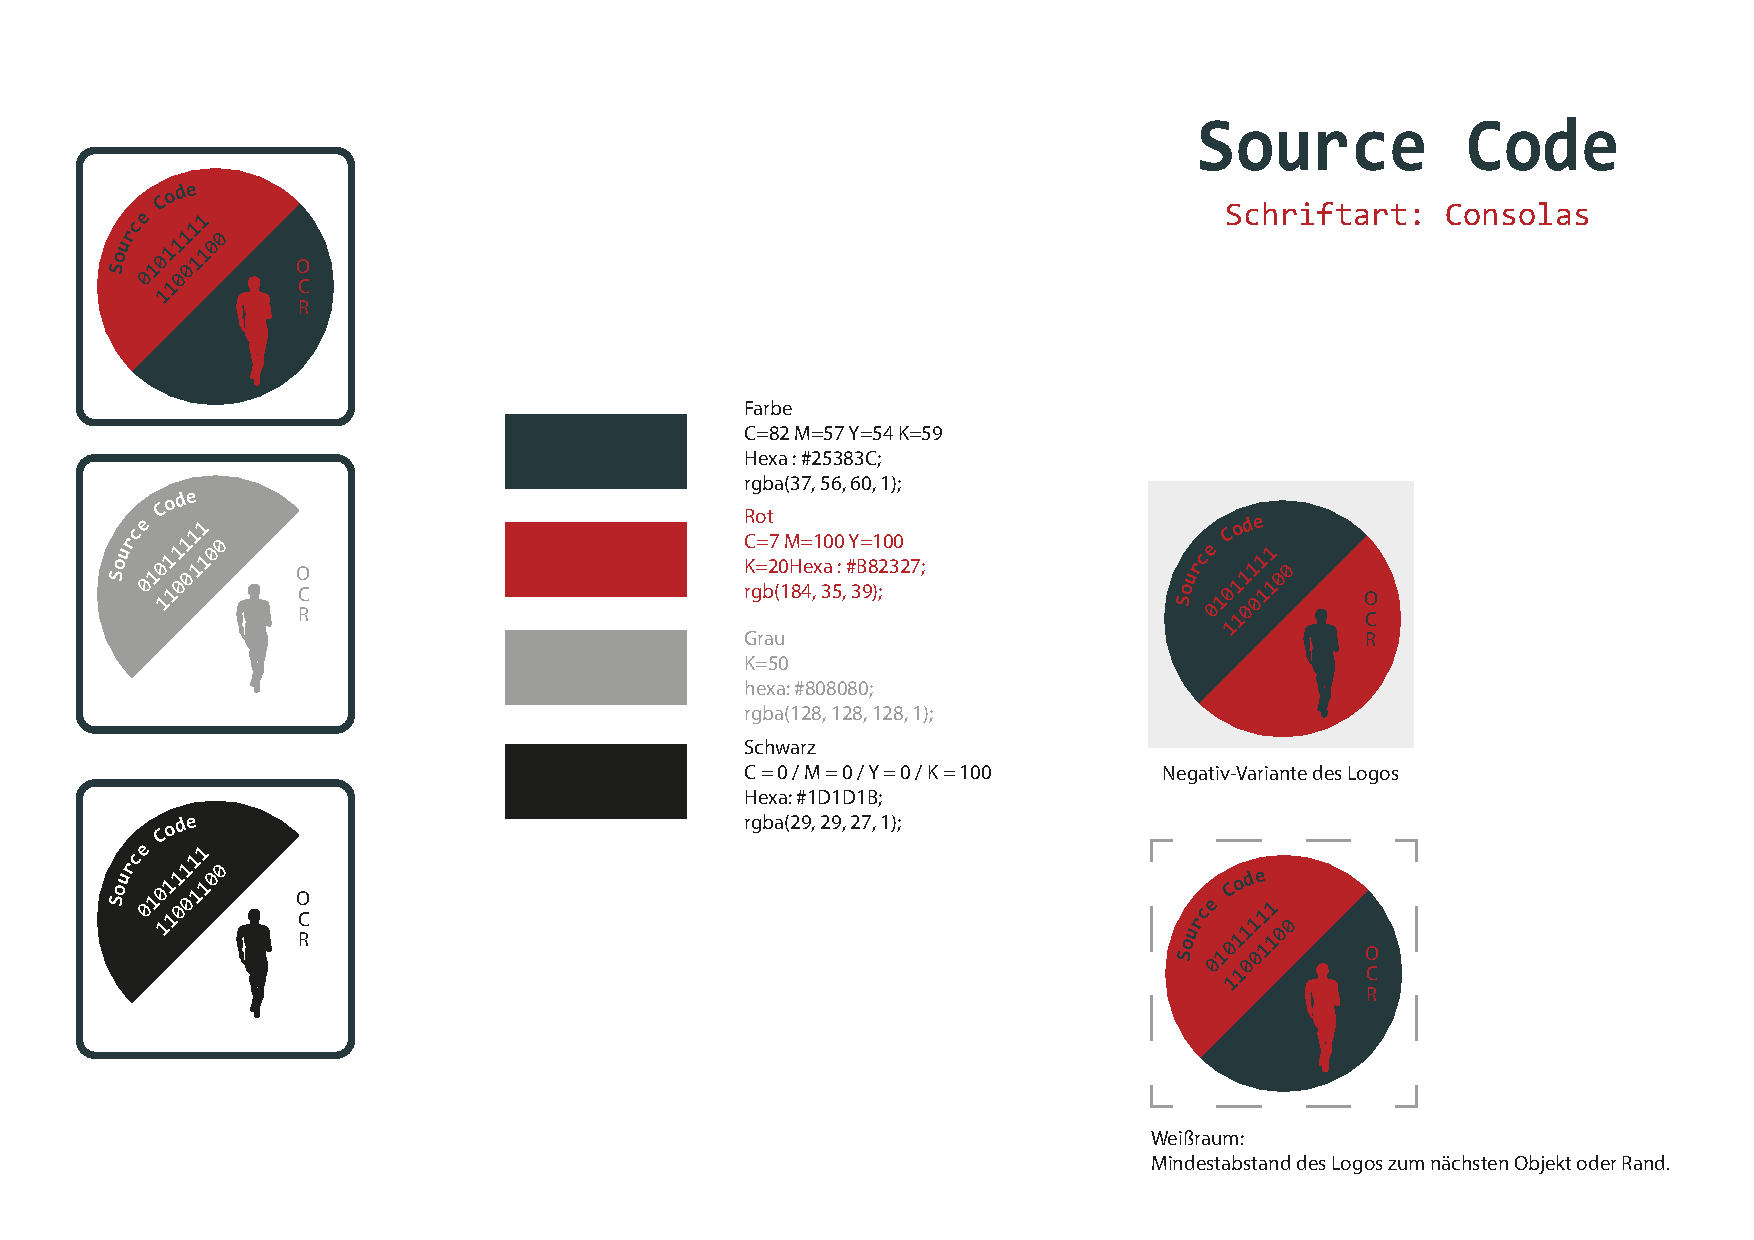
\includegraphics[width=.55\textwidth]{content/bsp/Logo-Details.pdf}
	\end{figure}

	\item Tabelle
	\newline 
	
	\begin{centering}
		\begin{tabular}[3] {| l | l | l |}
			\hline
			\textbf{Control Board Label} & \textbf{Wire Color} & \textbf{Signal} \\ \hline
			VCC & Red & Motor + \\ \hline
			GND & Black & GND \\ \hline
		\end{tabular} 	
	\end{centering}

	\item Werte

	\begin{itemize}
		\item \textbf{Temperature1:} ~ 30
		\item \textbf{M1/M2 Amps:} ~ 0.00
	\end{itemize}

\end{enumerate}

\begin{enumerate}
	\item Aufzählung
	\item Aufzählung
	\item Clone the code repo:
	\begin{enumerate}
		\item git clone https://github.com/ju-bw/notizenDummyWin10-v03.git 
		\item git checkout master
		\item git pull
	\end{enumerate}
\end{enumerate}

\begin{itemize}
	\item Punkt
	\item Punkt
\end{itemize}

\begin{enumerate}
	\item[] Direct downloadable Raspbian Buster image: 
	\item[] \href{https://downloads.raspberrypi.org/raspbian/images/raspbian-2019-07-12/2019-07-10-raspbian-buster.zip}{https://downloads.raspberrypi.org/raspbian/images/raspbian-2019-07-12/2019-07-10-raspbian-buster.zip}
\end{enumerate}


\subsection{Referenz und Links}
\label{referenz_links}

\begin{itemize}
	\item Link \href{https://www.ju1.eu/}{https://www.ju1.eu/}.
	\item \href{https://www.ju1.eu/}{Website}.
	\item File (siehe \href{https://github.com/ju-bw/dummy-Notiz-Win10-v03/Readme.pdf}{/Readme.pdf})
	\item Bild (siehe Abb. \ref{bild})
	\item Tabelle (siehe Tab. \ref{komponenten})
	\item Kapitel (siehe Kap. \ref{latex})
	\item Textfußnote \footnote{Fußnote}.
\end{itemize}


\subsection{Bilder}
\label{bilder}

%Bild (siehe Abb. \ref{bild})
\begin{figure}[H]
	\centering
	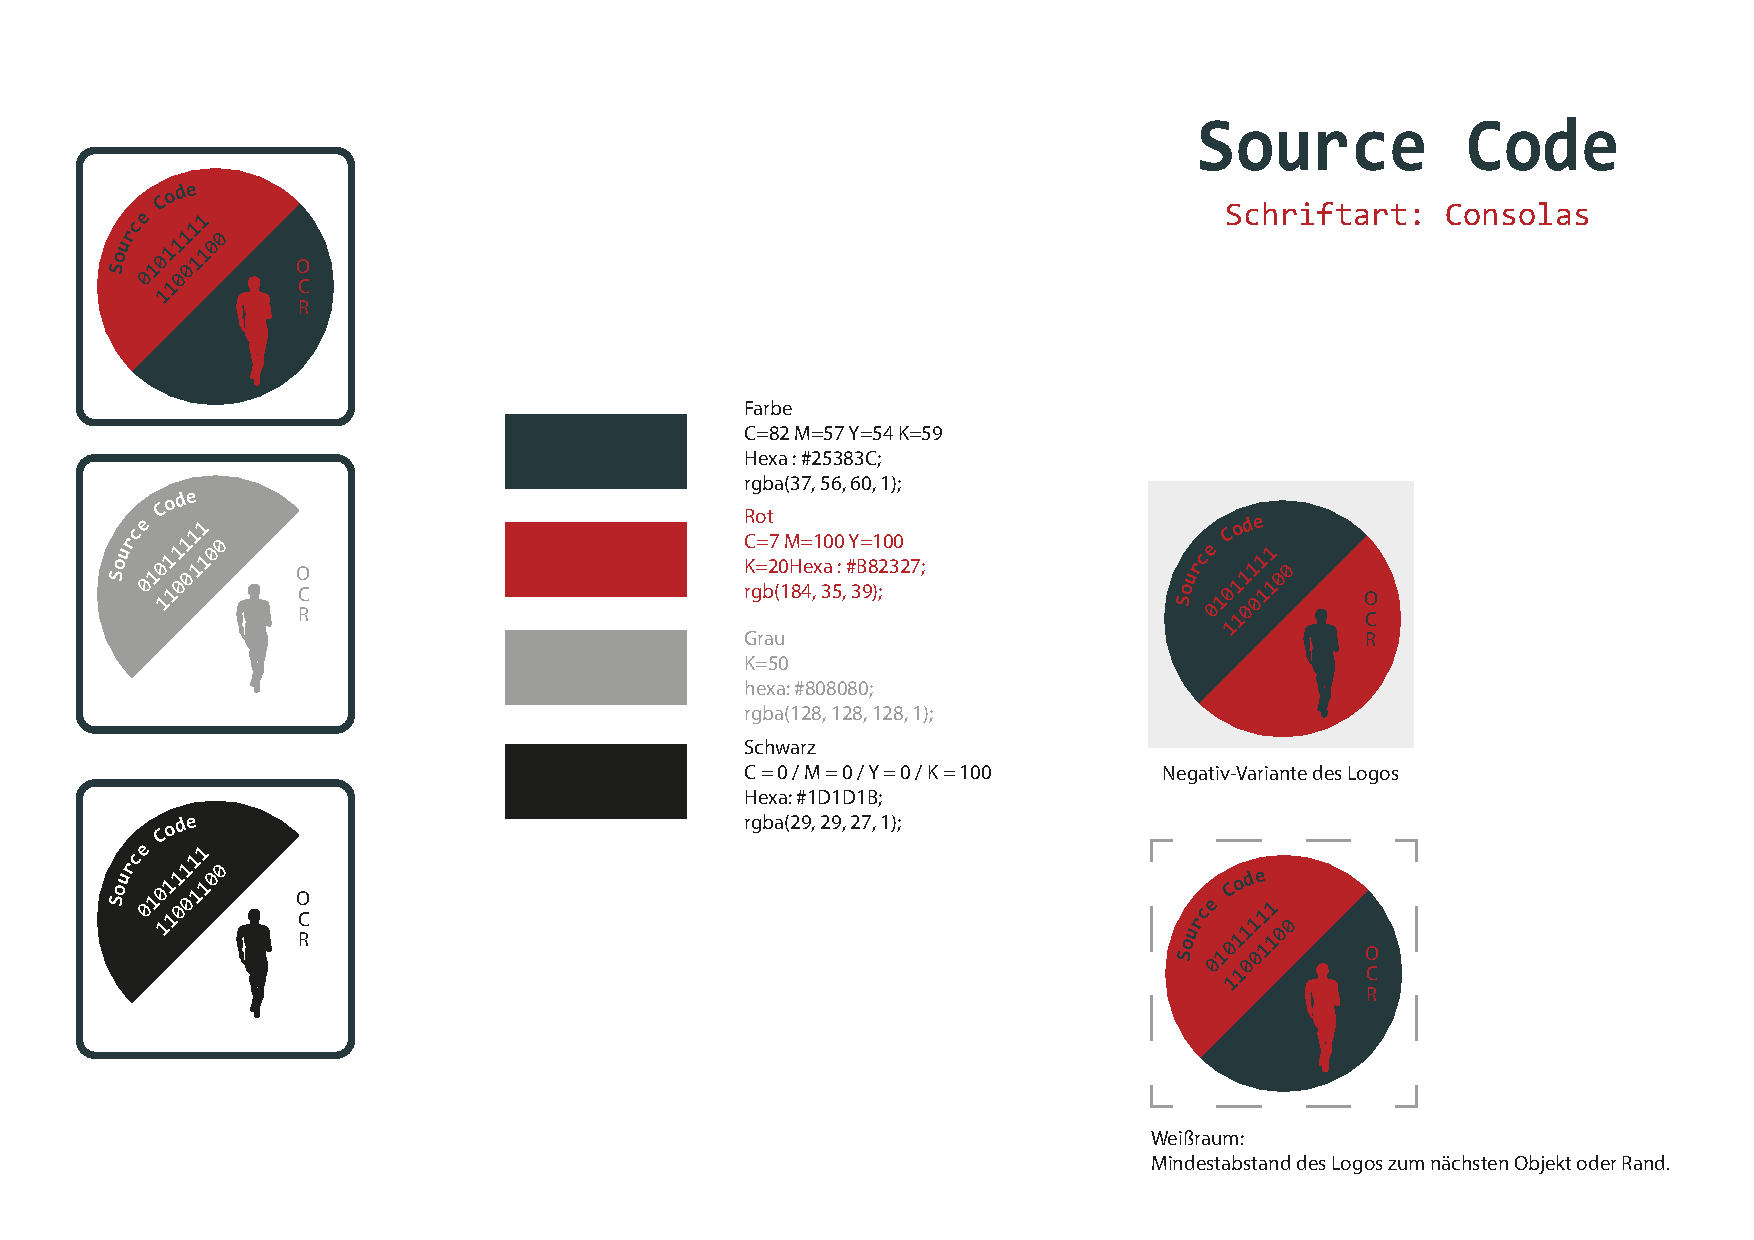
\includegraphics[width=.55\textwidth]{content/bsp/Logo-Details.pdf}
	%---------------------------------
	\caption{Bild} \label{bild}
\end{figure}

\begin{figure}[H]
	\centering
	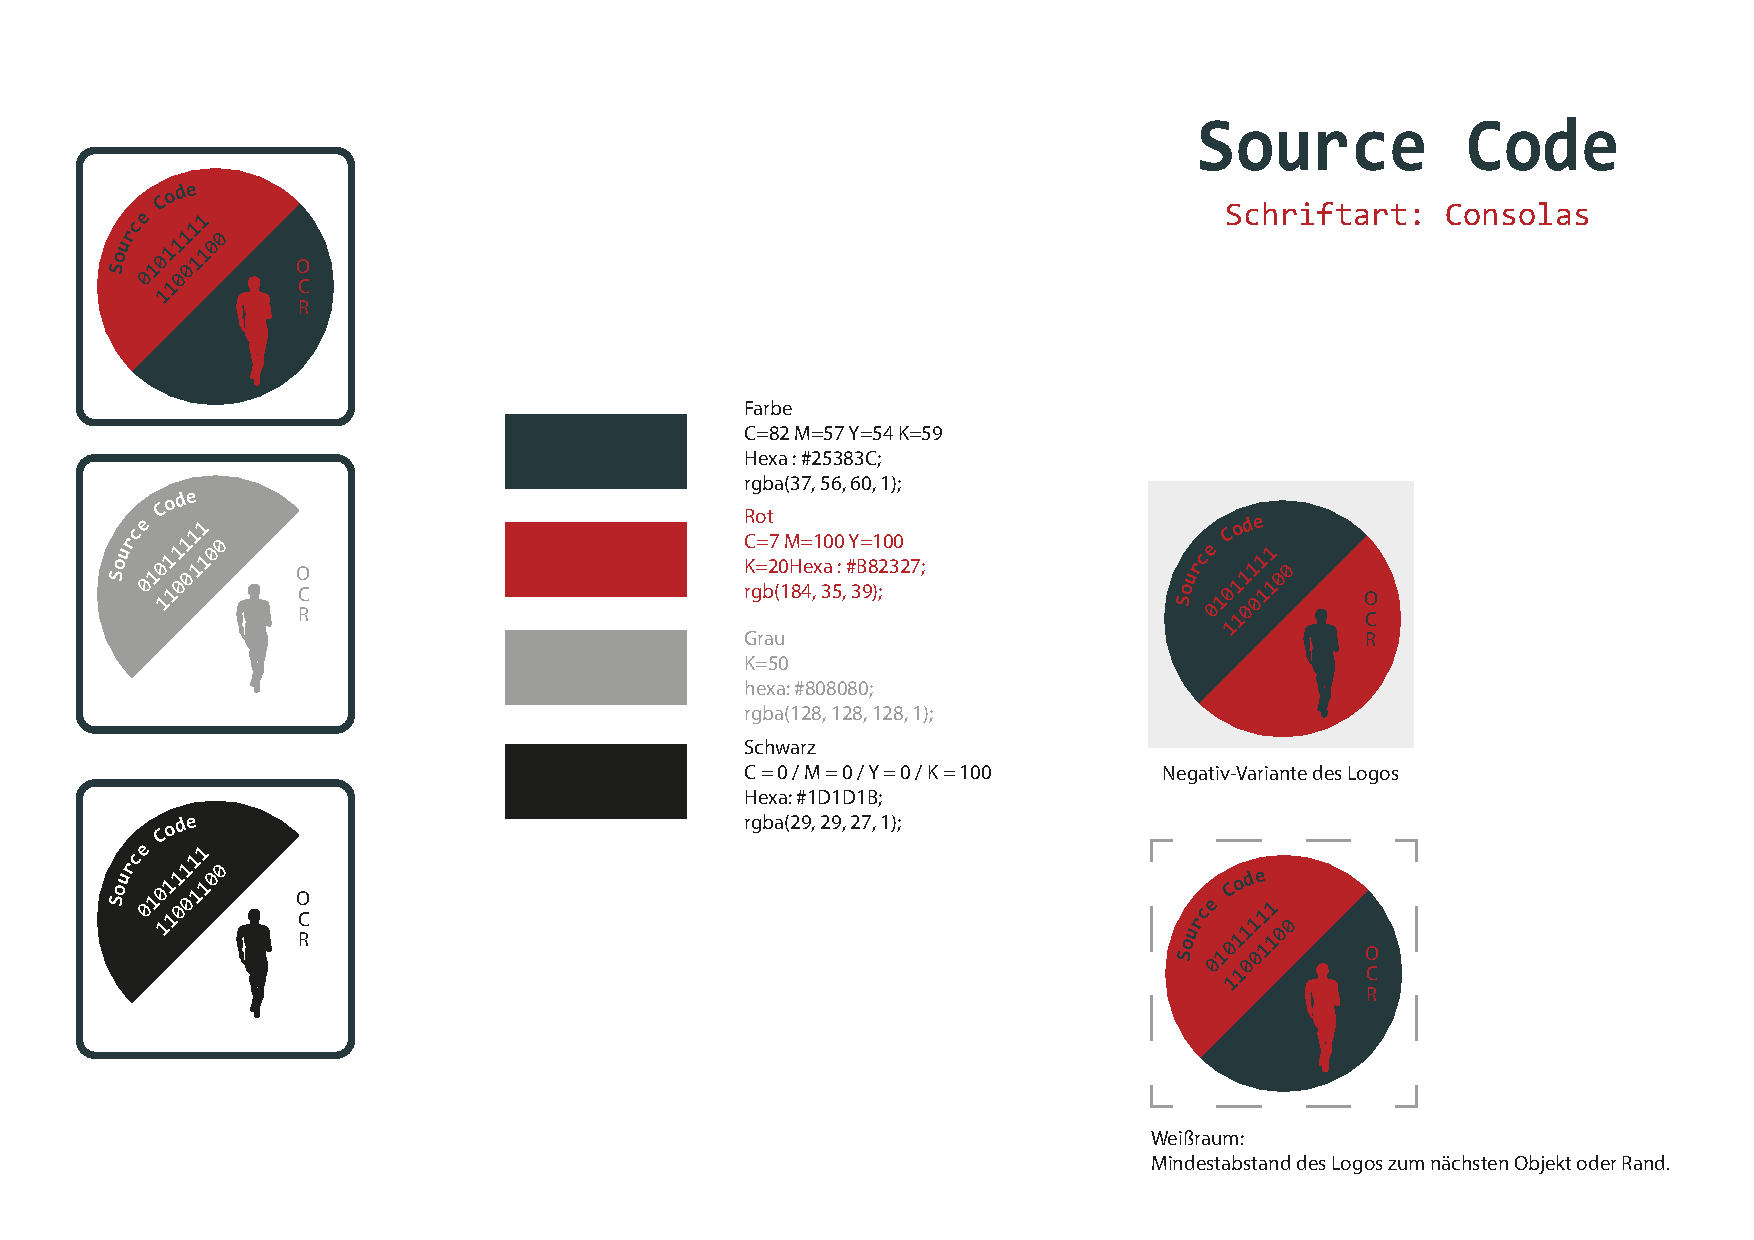
\includegraphics[width=.35\textwidth]{content/bsp/Logo-Details.pdf}
	%---------------------------------
	%\caption{Bild} \label{bild}
\end{figure}

Logo in Negativ, Grau u. Schwarz (siehe Abb. \ref{logo_negativ_grau_schwarz})
\begin{figure}[H]
	\centering
	\begin{minipage}[b]{0.40\textwidth}
		
\includegraphics[width=\textwidth]{content/bsp/Logo-negativ.pdf}
	\end{minipage}
	\hfill
	\begin{minipage}[b]{0.30\textwidth}
		
\includegraphics[width=\textwidth]{content/bsp/Logo-Grau.pdf}
	\end{minipage}
	\hfill
	\begin{minipage}[b]{0.20\textwidth}
		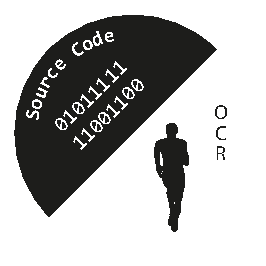
\includegraphics[width=\textwidth]{content/bsp/Logo-SW.pdf}
	\end{minipage}
	%---------------------------------
	\caption{Logo in Negativ, Grau u. Schwarz
		     \newline Quelle: https://www.ju1.eu/}
	\label{logo_negativ_grau_schwarz}
\end{figure}

Logo Details (siehe Abb. \ref{logo_details})
\begin{figure}[H]
	\centering
	\begin{minipage}[b]{0.49\textwidth}
		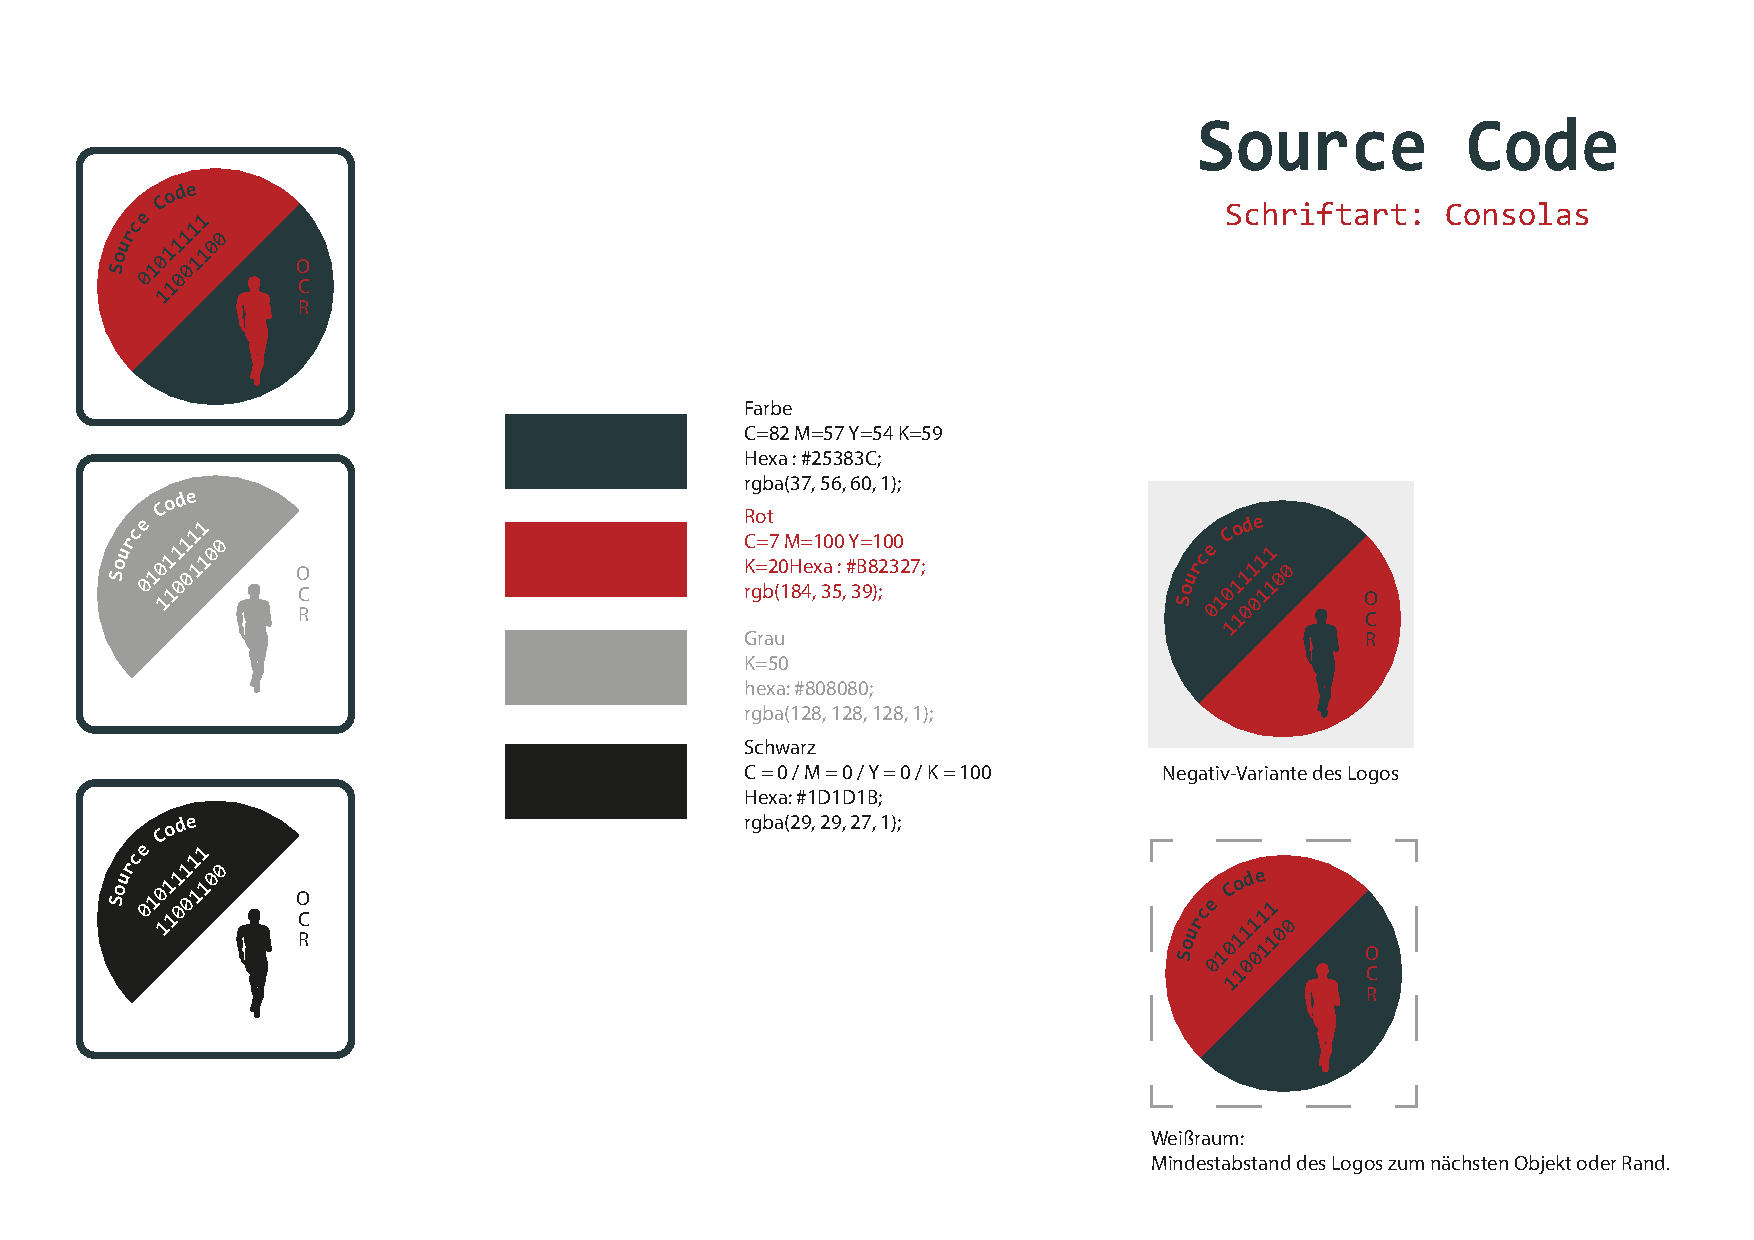
\includegraphics[width=\textwidth]{content/bsp/Logo-Details.pdf}
	\end{minipage}
	\hfill
	\begin{minipage}[b]{0.49\textwidth}
		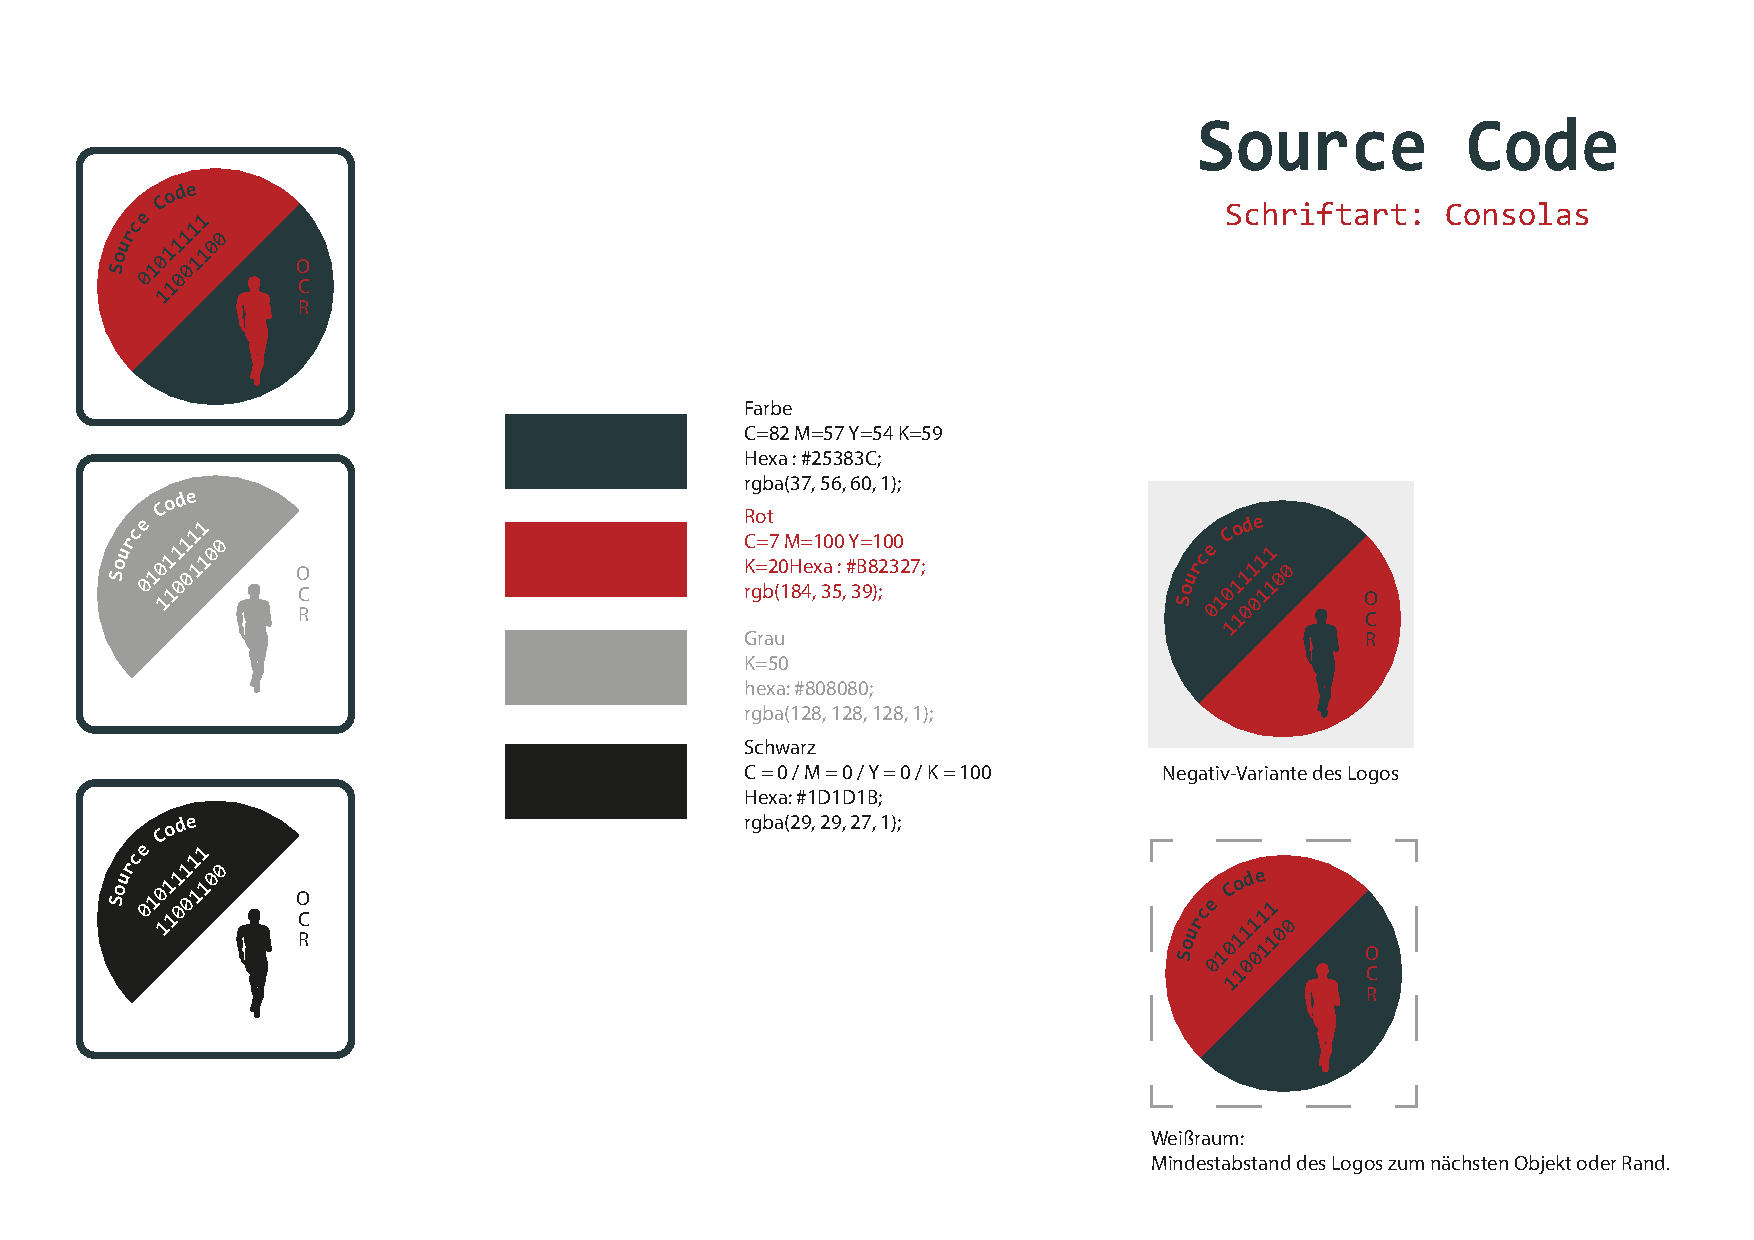
\includegraphics[width=\textwidth]{content/bsp/Logo-Details.pdf}
	\end{minipage}
	%---------------------------------
	\caption{Logo Details} \label{logo_details}
\end{figure}


\subsection{Tabelle}
\label{tabelle}

Tabelle (vgl. Tab. \ref{tabelle_}). 
\begin{table}[H]% hier: htbp
	\centering
	\arrayrulecolor{lightgray}
	\sffamily\footnotesize
	\begin{tabular}{ll}% Spalte: lcr 
		\toprule
		\textbf{Nr.} & \textbf{Vorgehen} \\
		\midrule
		1 & Aktuellen Forschungsstand recherchieren \\
		2 & Methoden entwickeln \\
		3 & Schlussfolgerung aufstellen \\
		\bottomrule
	\end{tabular}
	%---------------------------------
	\caption{Tabelle}\label{tabelle_}%
\end{table}

\bigskip
%\centering
\begin{tabular}[2]{|p{3cm}|p{9cm}|}
	\hline
	\textbf{Teil} & \textbf{Beschreibung} \\ \hline
	Batterie & Versorgt das System mit Strom. Hat einen ungeregelten Spannungsbereich von ca. 11,5 V - 16,75 V je nach Ladezustand \\ \hline
	Schalter & mechanische Trennung der elektrischen Energie zum Rest des Roboters \\ \hline
\end{tabular}
\bigskip

%\centering
\begin{tabular}[3] {| l | l | l |}
	\hline
	\textbf{Control Board Label} & \textbf{Wire Color} & \textbf{Signal} \\ \hline
	VCC & Red & Motor + \\ \hline
	GND & Black & GND \\ \hline
\end{tabular} 
\bigskip

%\centering
\begin{tabular}{|N|N|}
	\hline
	\textbf{Control Board pin} & \textbf{cable wire color} \\ \hline
	1. GND & Black \\ \hline
	2. 5V & Red \\ \hline
\end{tabular}
\bigskip

\begin{table}[H]
	\centering
	\arrayrulecolor{lightgray}
	\sffamily\footnotesize
	\begin{tabular}{|N|Q|Q|I|N|Q|Q|I|}
		\hline
		\thead{Artikel} & \thead{Ref} & \thead{Menge} & \thead{Bild} & 
		\thead{Artikel} & \thead{Ref} & \thead{Menge} & \thead{Bild} \\ \hline
		Battery & logo & 1 & \partimg{content/bsp/logo.pdf} & 
		Tamiya Connectors & logo & 1 & \partimg{content/bsp/logo.pdf} \\ \hline
		Battery Charger & logo & 1 & \partimg{content/bsp/logo.pdf} & & & & \\ \hline
	\end{tabular}
	%---------------------------------
	\caption{Komponenten} \label{komponenten}
\end{table}

\begin{table}[H]
	\centering
	\arrayrulecolor{lightgray}
	\sffamily\footnotesize
	\begin{tabular}[3] {| p{2cm} | p{5cm} | p{2cm} | }
		\hline
		\textbf{Pin} & \textbf{Description} & \textbf{Color} \\ \hline
		1 & +5V DC Power & \textcolor{red}{\textbf{Red}} \\ \hline
		2 & GND & \textcolor{black}{\textbf{Black}} \\ \hline
	\end{tabular}
	%---------------------------------
	\caption{Pinbelegung} \label{pinbelegung}
\end{table}

\begin{table}[H]
	\centering
	\arrayrulecolor{lightgray}
	\sffamily\footnotesize
	\begin{tabular}{|c|c|c|}
		\hline
		\thead{Item} & \thead{Ref} & \thead{Board Ref} \\ \hline
		4.7K 1/4 Watt Res & E7 & R1 \\ \hline
		10K 1/2 Watt Res & E10 & R2 \\ \hline
		100nF Cap & E11 & C1-17 \\ \hline
	\end{tabular}
	%---------------------------------
	\caption{Resistor/Capacitor reference}
\end{table}

\begin{centering}
	\begin{tabular}[2]{|c|c|}
		\hline
		\textbf{Variable} & \textbf{Physical description} \\ \hline
		$d_1$ & Horizontal distance \\ \hline
		$d_2$ & Vertical distance  \\ \hline
	\end{tabular}
	
	\begin{figure}[H]
		\centering
		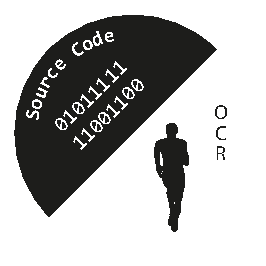
\includegraphics[width=.35\textwidth]{content/bsp/Logo-SW.pdf}
		%---------------------------------
		\caption{Physical distance} \label{r5}
	\end{figure}	
\end{centering}

\subsection{Formel}
\label{formel}

\begin{equation}
	d_1 = 7.254 mm \qquad d_2 = d_3 = 10.5 mm \qquad d_4 = 10.073 mm
\end{equation}

\begin{equation}
	1 \le 2 \ge 0 \neq 4, \quad 1 \ll 10^{20} \gg 10^{-5} \pm 
\end{equation}

\begin{equation}
	a \cdot b \quad
	a \times b \quad
	\frac x2 \quad
	a_1 \quad
	a^2 \quad
	\binom{a}{b} \quad
	\sqrt{x} \quad bzw. \quad \sqrt[n]{x} \quad	
\end{equation}

\begin{equation}
	\sum \limits_{i=1}^n i = \frac{n(n+1)}{2}
\end{equation}

\begin{equation}
	\prod \limits_{i=1}^{n+1}i = 1\cdot 2\cdot\dots\cdot n\cdot (n+1)
\end{equation}

\begin{equation}
	\lim\limits_{n \to \infty}\frac{1}{n}=0
\end{equation}

\begin{equation}
	\left(
		\begin{array}{ccc}
			a_{11} & \cdots & a_{1n} \\
			\vdots & \ddots & \vdots \\
			a_{m1} & \cdots & a_{mn}
		\end{array}
	\right)	
\end{equation}

\subsection{Textauszeichnung}
\label{textauszeichnung}

\textbf{fetter Text}

\textbf{**Hinweis** Diese haben NICHT die gleiche Farbe und Pinbelegung wie die Antriebsmotoren!}


\subsection{Farben}
\label{farben}

\begin{itemize}
	%\textcolor{}{}
	%\item[] \colorbox{}{}
	\item[] \colorbox{Apricot}{Apricot} \colorbox{Aquamarine}{Aquamarine}
            \textcolor{Apricot}{Apricot}
	\item[] Apricot		Cyan		Mahogany		ProcessBlue		SpringGreen
	\item[] Aquamarine		Dandelion		Maroon		Purple		Tan
	\item[] BitterSweet		DarkOrchid		Melon		RawSienna		TealBlue
	\item[] Black		Emerald		MidnightBlue		Red		Thistle
	\item[] Blue		ForestGreen		Mulberry		RedOrange		Turquoise
	\item[] BlueGreen		Fuchsia		NavyBlue		RedViolet		Violet
	\item[] BlueViolet		Goldenrod		OliveGreen		Rhodamine		VioletRed
	\item[] Brickred		Gray		Orange		RoyalBlue		White
	\item[] Brown		Green		OrangeRed		RoyalPurple		WildStrawberry
	\item[] BurntOrange		GreenYellow		Orchid		RubineRed		Yellow
	\item[] CadetBlue		JungleGreen		Peach		Salmon		YellowGreen
	\item[] CarnationPink	Lavender	Periwinkle	SeaGreen YellowOrange
	\item[] Cerulean		LimeGreen		PineGreen		Sepia
	\item[] CornflowerBlue	Magenta	 Plum	SkyBlue
\end{itemize} 


\subsection{Zusammenfassung}
\label{zusammenfassung}

\mybox{
	Es gibt ein paar wichtige Dinge, die beachtet werden sollten, wie bei jedem Projekt, bei dem mit Batterie oder elektrischem Strom gearbeitet wird:
	\newline
	\noindent \textbf{DIE BATTERIE}. 
}